\documentclass[letterpaper]{article}
\usepackage{natbib,reddit-sa}
\usepackage{filecontents,lipsum}
\usepackage{array}

\makeatletter
\renewcommand{\fnum@figure}{Fig. \thefigure}
\makeatother

\title{2016 U.S. Presidential Election - Reddit Comment Temporal and Sentiment Analysis}
\author{Connor Griep$^{1}$, Jacob Shiohira$^{1}$, \and Jacob Warner$^{1}$ \\
\mbox{}\\
$^1$University of Nebraska-Lincoln, $1400$ R St, Lincoln, Nebraska \\
\mbox{}\\
connorgriep@gmail.com \\
jacob.shiohira@huskers.unl.edu \\
jwarner@huskers.unl.edu }


\begin{document}
\maketitle

\section{I. INTRODUCTION}

% make this indent?
The 2016 presidential election was one of the most heated elections to date. The tone of the election campaign was generally characterized as divisive and negative, with both candidates surrounded with immense controversy. There was no way that both sides were going to be satisfied, but there is not a definitive source saying how the general population reacted to the events of the election. Reddit, a social media platform, has an active political community that is rich in information about the public's attitudes and feelings towards political topics and candidates. This project’s temporal sentiment analysis approach should be able to capture some interesting information regarding the attitude and feelings of the U.S. electorate over the month surrounding the election (October 25, 2016 to November 22, 2016). The election of the president is one of the most important events in the U.S. Being such an important event, we believe it’d be fascinating to explore America’s reaction throughout the election process. More specifically, we are interested in how people’s attitudes and interactions changed as it became more apparent that Donald Trump was a serious competitor.

Reddit allows users to post under unvalidated and anonymous accounts, which some argue allow people to post true feelings and opinions, as opposed to sites like Facebook where family and friends are likely to see whatever users post, causing them to hide or restrict their truest thoughts. Reddit’s data is invaluable for our project because it’ll allow us to better analyze the sentiment and emotion behind each comment, making the end result much more accurate in terms of how people really felt about the election.

There is an overwhelming amount of Reddit comment data dating from December 2005 to today. There are roughly 10,000 JSON objects representing comments per megabyte. Thus, in a monthly average of 6GB of data, there is approximately 60 million comments. We are only looking at 2 weeks before and after the 2016 election, which limits the total comments we work with to around 60 million. By looking at the month surrounding the election, we believe we’ll find the most interesting change in emotion compared to looking over the entirety of the election. It’ll also allow us to reduce the intense load of data we’re analyzing.

Contributions from this project to the overall data mining community will be limited since it will not propose any new algorithmic techniques. However, this project’s contribution will primarily be its unique approach to extracting data around a specific, major event. The Reddit comment dataset is incredibly large, so narrowing the scope of interest allows one to ask specific questions, which comments and their respective feelings and emotions could provide insight to.

The data set for this project has access to every Reddit comment made publically available from December 2005. The approach this project uses could then be applied to any major event since 2005 using any collection of subreddits. For example, we could explore how subreddits in the business and economic categories reacted to the 2009 housing market crash by applying this approach. Furthermore, this approach could be applied to examine if major events have any effect on seemingly unrelated topics. For instance, to see if the Superbowl for American football has any effects on general sentiment of comments made in a subreddit for financial investing. Lastly, this approach could also be extended to any social media platform that includes the ability for users to interact via comments. Different comment datasets from Youtube, Facebook, or Twitter could be used to determine the sentiment effects of certain videos, topics, or tweets. The results may vary between social media sites due to factors such as anonymity , but that’d also be an interesting result within itself.


\section{II. OBJECTIVES}
\begin{itemize}
    \item Data acquisition and cleaning (bots, moderators, etc.)
    \begin{itemize}
        \item Acquisition - JSON to Database program - automation
        \item Cleaning - bots and moderator filter
        \item Cleaning - subreddit filter - start with a specific number of political subreddits
    \end{itemize}
    \item Sentiment analysis
    \begin{itemize}
        \item Submit comment text to Sentiment Analysis API’s to classify the sentiment of the comment as a whole
    \end{itemize}
    \item Associate words with emotion
    \begin{itemize}
        \item Dates around the election, broken up into 2 weeks before (WB), 1 WB, 1 day before, the day of the election, 1 day after, 1 week after (WA), 2 WA
        \item Time of Election Day: Morning to afternoon to night
    \end{itemize}
\end{itemize}

\section{III. RELATED WORK}

\subsubsection{Opinion Mining and Sentiment Analysis}
This project used term presence vs frequency, position, and parts of speech information, syntax, and negation to analyze comments on various review sites. Specifically looking at political sites, they found that $31\%$ of Americans gathered information about the $2006$ election on the internet and exchanged views via email. Of this $31\%$, many were seeking perspectives from inside their community ($28\%$) and outside their community ($34\%$), \cite{OpinionMining}. With the increased use of both the internet and review sites with a comment section, the same statistics for the $2016$ election are likely much higher.
% lessons learnt
This paper shows that there is a market for political analysis. It has been shown that the internet is a valid platform for people to converse and sway opinions. In doing so, the emotions of posts might change and that is what we are trying to discover with our project.
% how ours is different
The research in the paper focused on personal blogs and review sites. This could have different results from a forum based site like Reddit.

\subsubsection{Sentiment Analysis on News Comments based on Supervised Learning Method}
This paper collected news comments hoping to improve the sentiment classification. They compared feature selection methods, feature representation methods, and classifiers of sentiment classification, \cite{SentimentAnalysis}. They found that document frequency, importance of feature, and relevance between features were effective feature selection methods for every classifiers. 
% lessons learnt
There are a variety of ways to classify sentiment to have the best results. Our project should look into these methods and determine which ones are best fit for our problem statement.
% how ours is different
Our project focuses on comments instead of review pieces. It could be more difficult to find the correct sentiment classification method for comments as they are just responses to a topic rather than reviews which have the sole purpose of trying to sway the readers with a certain opinion.

\subsubsection{Large-Scale Sentiment Analysis for News and Blogs}

This paper assigned a score to newspaper and blog pieces that expressed opinions about recent events. They wanted to find the positive or negative opinion on each entity presented (people, places, things)  in the piece of writing, \cite{LargeScaleSentiment}. They used sentiment lexicons in conjunction with path analysis in order to evaluate the overall feeling generated by the writing. A final score (to determine overall feeling) would be given only to paths that met their threshold value.
We should look at the same methods as this approach helps with finding an emotion for difficult words that have different connotation. For example, “shoot” can be good seen as good or bad in the sentences, “shoot the bad guy” (good) and “shoot the good guy” (bad).
The research paper has the same general idea as us, but looks at newspaper and blog posts instead of comments. It is much easier to identify the entities in a post because they are required in order to make a coherent post. A comment is not required to include people, places, or things to still make sense.

\section{IV. PROBLEM DEFINITION}

Reddit has an active community with copious amounts of unorganized information on the public's attitudes and feelings towards various events. There are few real world applications for all of this data regarding substantial events. This project will use sentiment analysis of politically related subreddits to explore the general attitude and emotions related to comments before and after the 2016 presidential election, as it was one of the most controversial elections to date. The total input scope of comments is two weeks before to two weeks after the election. The reddit comments will then be filtered by subreddit such that only political subreddits will be considered, including Politics, US Politics, American Politics, Democrats, Republicans, and 2016Elections. After running sentiment analysis on all relevant comments, the output will be various plots. Most notably, it will be interesting to plot the average sentiment of comments within various subreddits as the election approaches and then passes. Another interesting plot will be the relationship between comment sentiment and the total up and down votes to see if the subreddit community agrees with what is being posted.

Generally, the comments of prominent social media platforms surrounding major domestic or international events are interesting because they are a decentralized source of general public sentiment. Comments and interactions can be collected across physical location and time, which could yield unexpected correlations between events, public sentiment, and long term effects.

\section{V. DATA SET}
The data set for this project is the set of comments from Reddit.com from a specific number of subreddits during the two weeks before and two weeks after the 2016 Presidential election (October 25th to November 22nd). The total Reddit comments data set contains a total of more than 1.7 billion JSON objects.The data set was collected using the Reddit API because someone wanted to collect the publicly available comments for research purposes.  

Table $1$ shows the attributes chosen for this project. Each was chosen for a specific reason. The body will be the main piece used for the sentiment analysis. After the analysis is complete, it will be compared to the downs, or down votes (if a post is seen by the community as negative) and ups, or up votes (if the post is seen by the community as positive) for any correlations. The author attribute is unique and will be useful to determine how often people post a comment. We also want to know if a post is edited as that could interfere with the relationship to the up and down votes.

\begin{table}[!hbt]
\center{
\begin{tabular}{|c|c|}\hline
Attribute & Data Type \\ \hline\hline
ups & int \\
edited & boolean \\
controversiality & int \\
subreddit & string \\
body & string \\
created$\_$utc & int \\
downs & int \\
score & int \\
author & string \\ \hline
\end{tabular}
}
\caption{Data Set Attributes}
\end{table}


\section{VI. APPROACH}

Briefly describe what approach you are planning to use. What software systems, components do you plan to use? Use of schematics, flowcharts, or pseudocode often makes it easier to follow an algorithm/approach.

Text analysis is the process of derivation of high end information through established patterns and trends in a piece of text. Using cutting edge techniques of Deep Learning like Long Short Term Memory (LSTM), Recurrent Neural Networks (RNN), Convolutional Neural Networks (CNN), etc. ParallelDots Text Analysis APIs perform significantly better than traditional Natural Language Processing techniques. We plan on using their APIs to perform both sentiment and emotion analysis.

Sentiment Analysis is contextual mining of text which identifies and extracts subjective information in source material. The ParallelDots API gives us the opportunity to classify each individual Reddit comment as positive, neutral, or negative. However, sometimes the three classes of sentiment (positive, negative and neutral) are not sufficient to understand the nuances regarding the underlying tone of a comment. Thus, the Emotion Analysis tells whether the underlying emotion behind a message is: Happy, Sad, Angry, Excited, Sarcasm, or Fear.

Behind the Sentiment Analysis are LSTMs. LSTMs model sentences as chains of forget-remember decisions based on context. Whereas an RNN can overwrite its memory at each time step in a fairly uncontrolled fashion, an LSTM transforms its memory in a very precise way: by using using specific learning mechanisms for which pieces of information to remember, which to update, and which to pay attention to. This helps it keep track of information over longer periods of time.

\begin{figure}[!htb]
\begin{center}
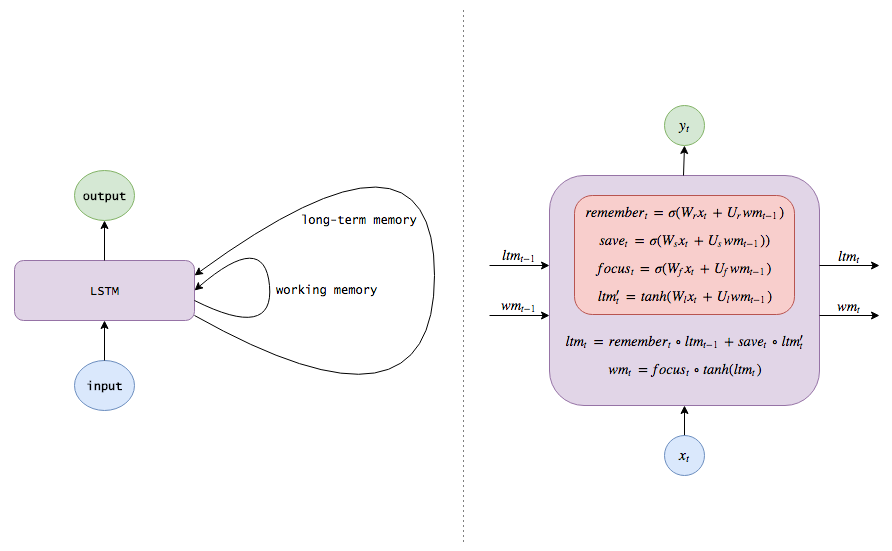
\includegraphics[width=3.4in]{lstm.png}
\caption{LSTM Neural Network Structure}
\label{fig1}
\end{center}
\end{figure}

% jank todo fix
\newpage

Behind the Emotion Analysis are CNNs. Emotions can be classified using extracted features of textual data, which are best extracted using CNNs.

\begin{figure}[!htb]
\begin{center}
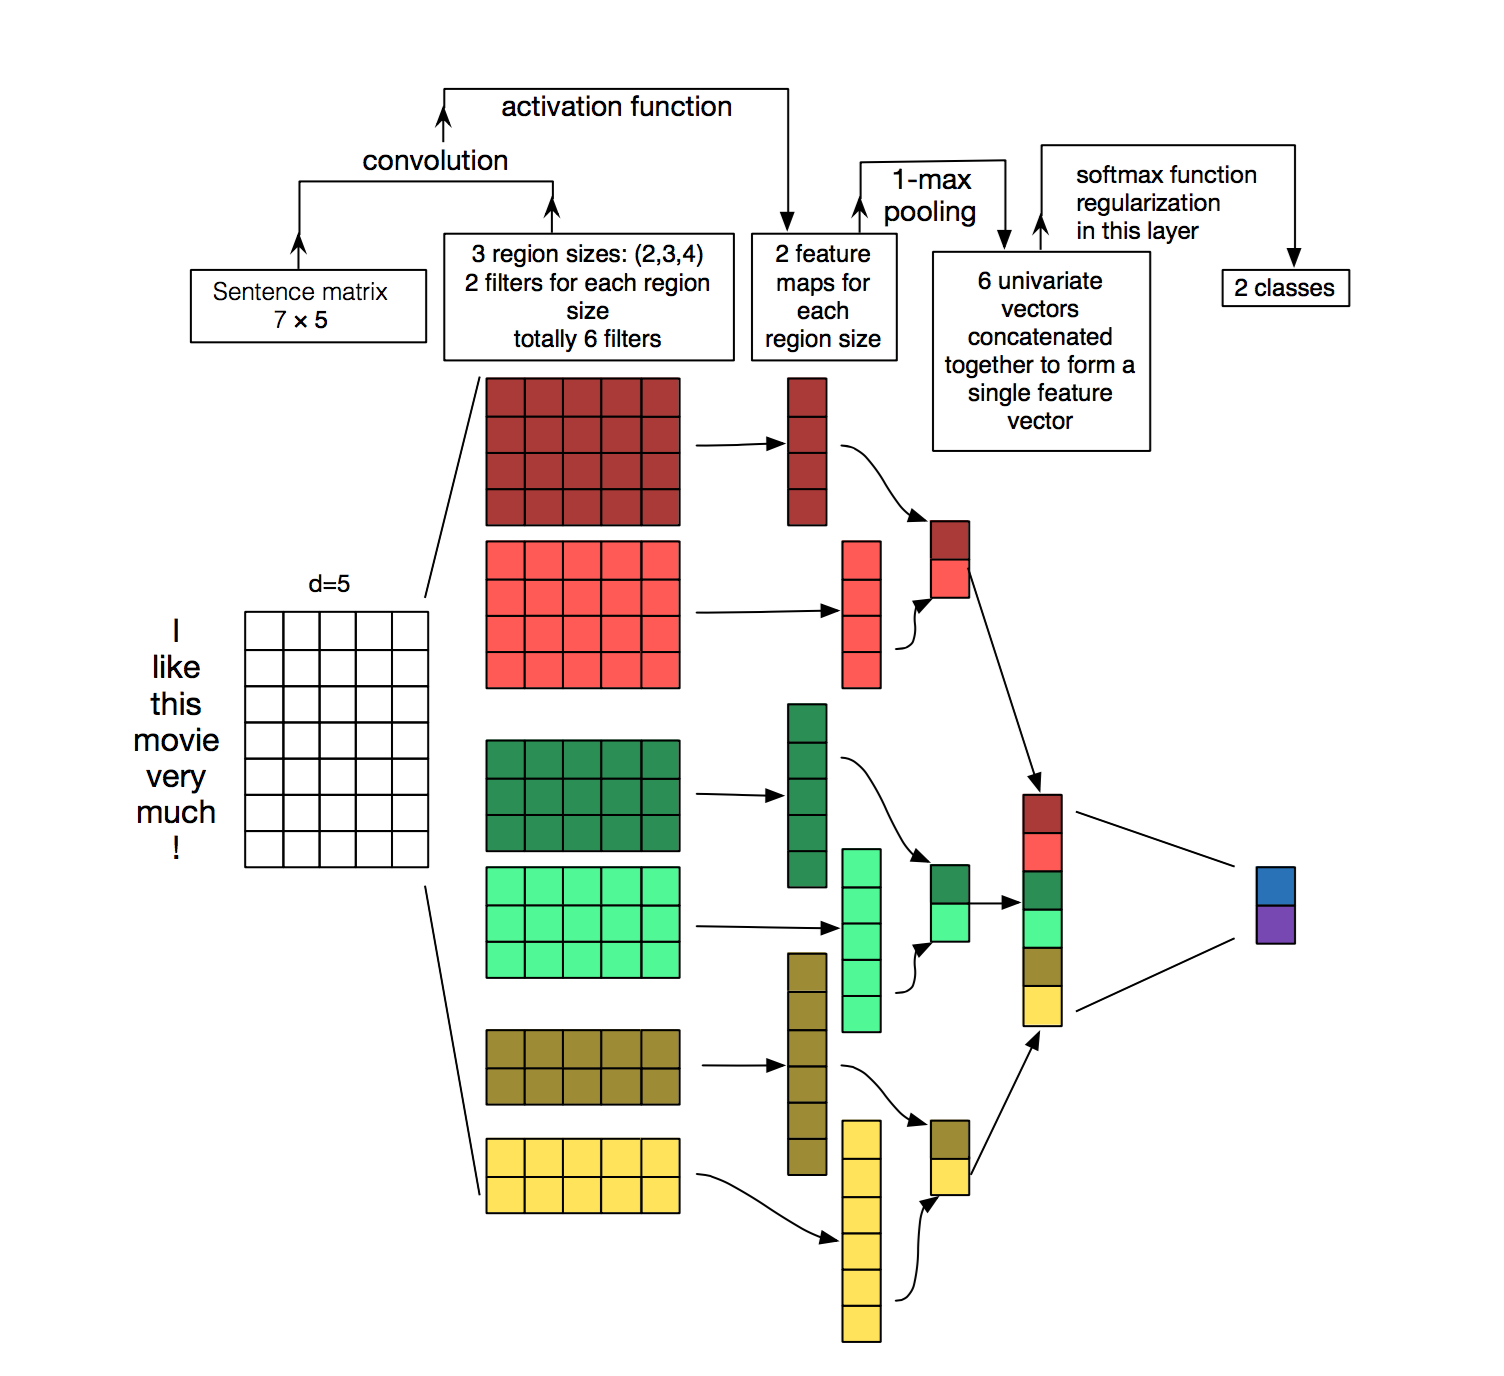
\includegraphics[width=3.4in]{cnn.png}
\caption{Convolutional Neural Network Structure}
\label{fig2}
\end{center}
\end{figure}

From each Reddit comment (JSON Object), the comment’s text will be extracted and passed to ParallelDots’ APIs. The Sentiment Analysis API returns a JSON Object of probabilities for the three classes sentiment, as well as the most prevalent sentiment. The Emotion Analysis API returns a JSON Object of probabilities for the underlying emotions, as well as the most prevalent emotion. The JSON Objects gathered from the API responses will be appended onto the end of the corresponding Reddit comment JSON Object for later use and analysis.

\section{VII. EVALUATION}

The evaluation of our approach will be later expanded. Currently, we will evaluate our approach based on the results found doing text and sentiment analysis. We cannot be certain about what we find as a result from analyzing, but a number of trends should be found. If the programs we use to analyze do not return consistent results that show trends we can be confident about, we will turn to alternative programs to find trends.

\section{VIII. IMPLEMENTATION PLAN AND TIMELINE}

\begin{center}
\begin{tabular}{ | l | c | } 
\hline
\textbf{Task} & \textbf{Date} \\ 
\hline
Completion of first objective &  March $30$ \\ 
\hline
Completion of second objective & April $9$ \\ 
\hline
Completion of third objective & April $16$ \\ 
 \hline
Finalize analysis and presentation & April $16$ to April $25$ \\ 
\hline
Presentation & April $25$ \\
\hline
Final report for this project & May $1$ \\ 
\hline
\end{tabular}
\end{center}

\footnotesize
\bibliographystyle{IEEEtran}
\bibliography{reddit-sa-bibliography}

\end{document}
